\chapter*{Affinity 2.0 settings for \gls{bc} vs \gls{ac} match test}
\label{apend:aff_bc_ac_match}
This appendix explain the settings for the Affinity 2.0 for \gls{bc} vs \gls{ac} matching.

\section*{Materials and setup}
To adjust the Affinity 2.0 settings, the following materials are used:
\begin{itemize}
\item Affinity 2.0
\item The Affinity 2.0 control computer with Affinity Suite
\end{itemize}

\begin{figure}[H]
	\centering
		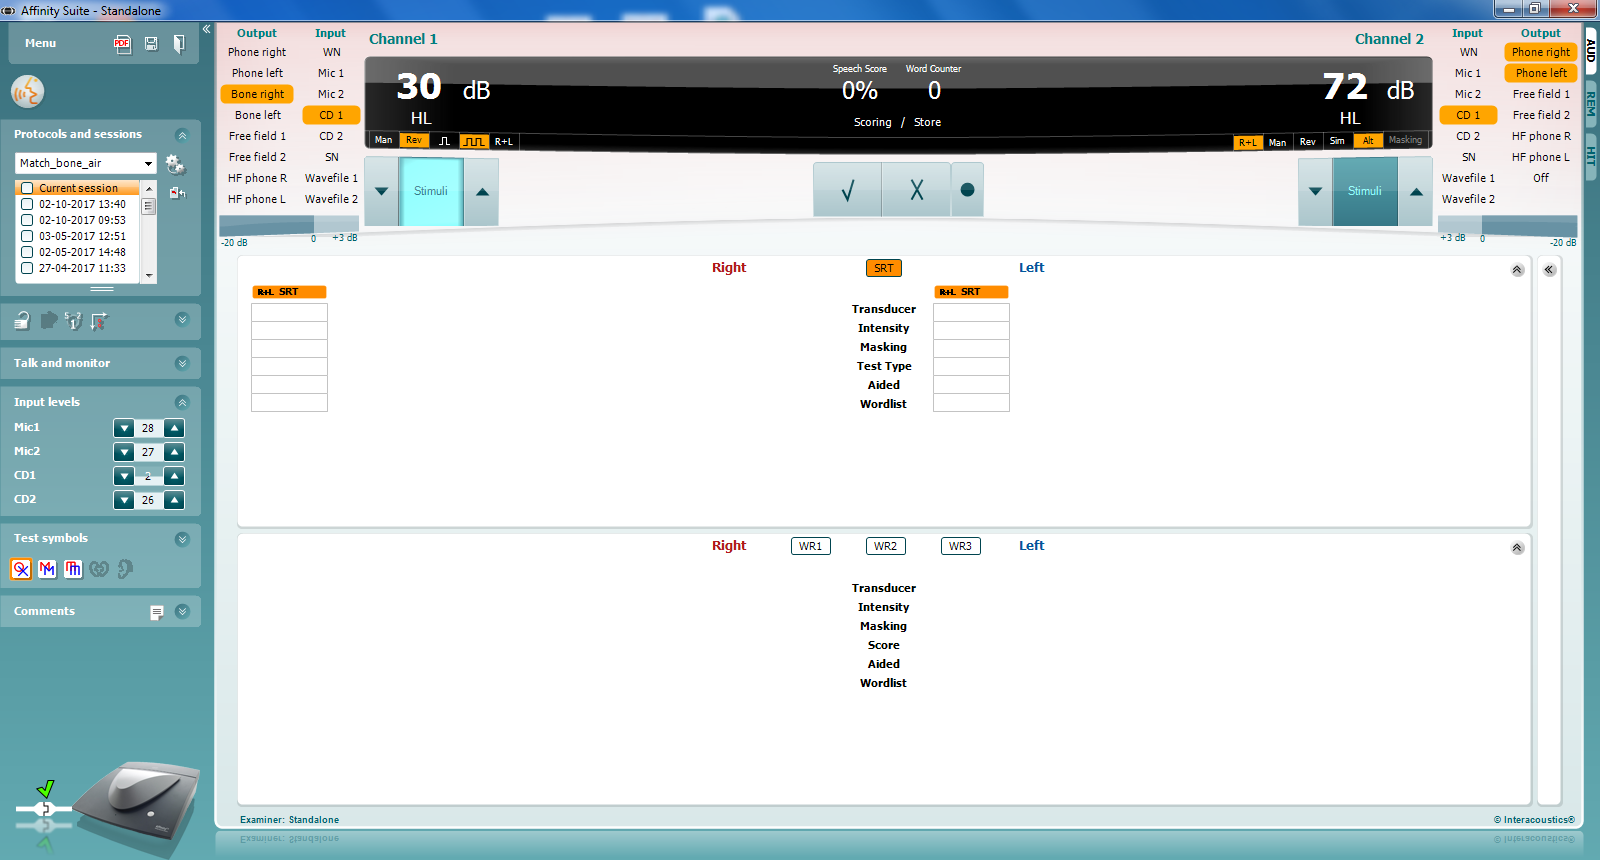
\includegraphics[width=1\textwidth]{match_bone_air}
		\caption{The settings for  \gls{bc} vs \gls{ac} matching}
		\label{fig:apend_match_bone_air}
\end{figure}

\section*{Test procedure}


\begin{enumerate}
\item The materials are set up as in \autoref{fig:appendix:test}.
\item 
\item  
\item  
\item 
\item 
\end{enumerate}

\chapter*{Affinity 2.0 settings for \gls{hint}}
This appendix explain the settings for the Affinity 2.0 forthe \gls{hint} test.

\section*{Materials and setup}
To adjust the Affinity 2.0 settings, the following materials are used:
\begin{itemize}
\item Affinity 2.0
\item The Affinity 2.0 control computer with Affinity Suite
\end{itemize}

\begin{figure}[H]
	\centering
		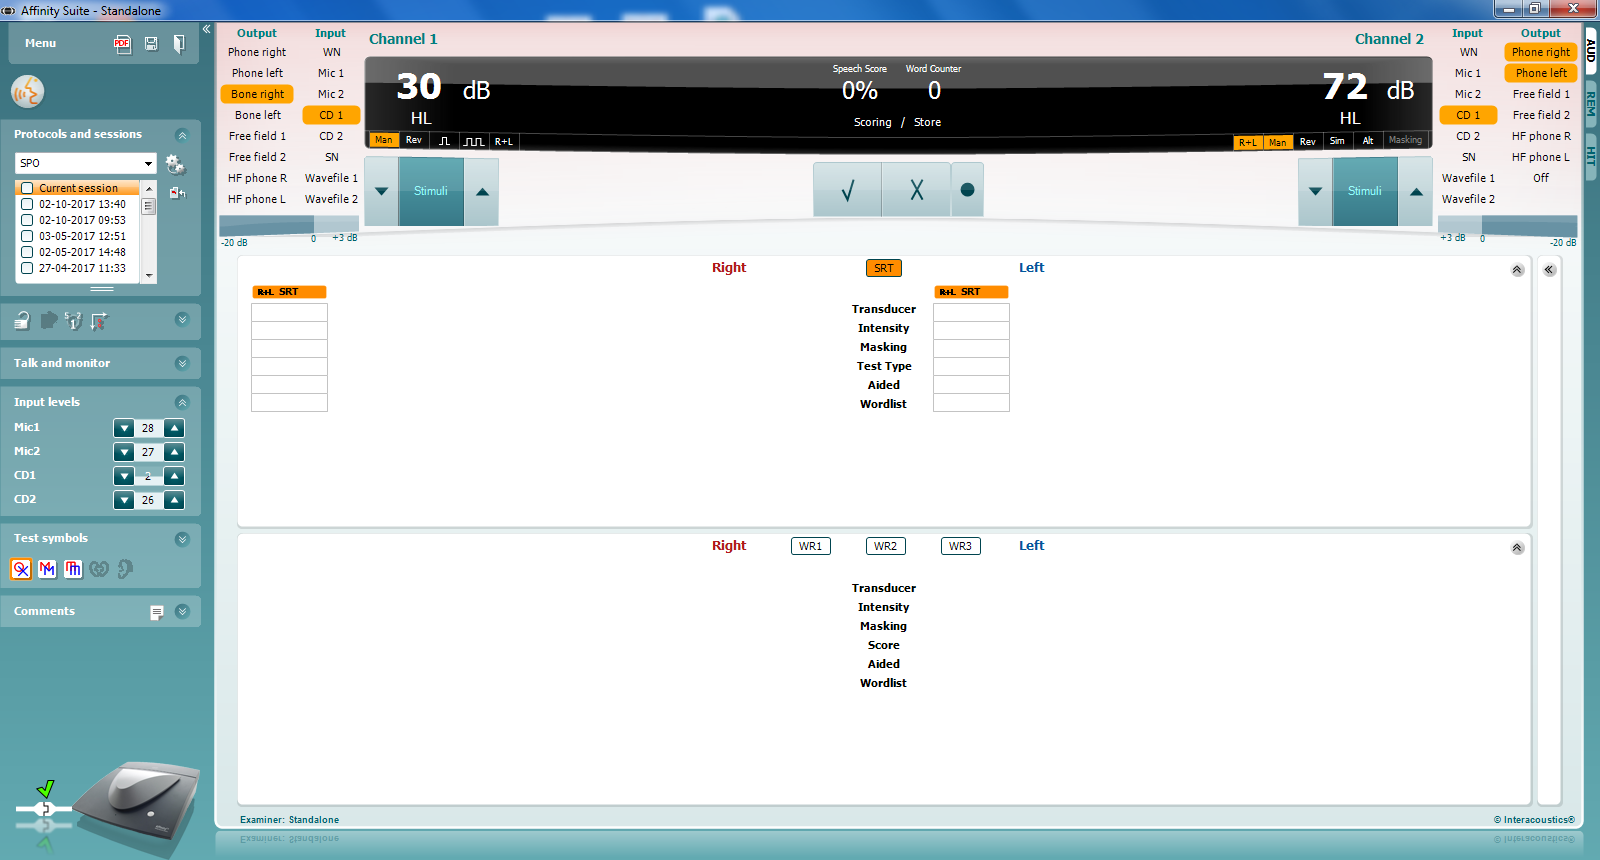
\includegraphics[width=1\textwidth]{spo}
		\caption{The settings for  \gls{hint} test}
		\label{fig:apend_match_bone_air}
\end{figure}

\section*{Test procedure}


\begin{enumerate}
\item The materials are set up as in \autoref{fig:appendix:test}.
\item 
\item  
\item  
\item 
\item 
\end{enumerate}
